\documentclass[12pt,draft]{article}
% draft - disables image rendering, shows black boxes at hyphenation issues
% Defaults:
%  10pt
%  notitlepage
%  usletter page size on some distros (not mine)
%  singleside (twoside changes the margins for a binding)

% Style:
% http://practicaltypography.com
% https://www.sharelatex.com/learn/Paragraphs_and_new_lines

% Left-aligned text; equal spacing between words, better readability
%  May look "unprofessional", books, articles typically use fully justified
% ragged2e retains hyphenation and attempts to give a more uniform right edge, but maintains equal spacing between words
\usepackage{ragged2e}
\RaggedRight

% Single space after a full stop, modern typographic readability standard
\frenchspacing

% Paragraph spacing with no indent; breaks up huge blocks of text
\usepackage{parskip}

% Line spacing (Default or slightly larger?)
%\usepackage{setspace}
%\onehalfspacing

% Header and footer
\usepackage{fancyhdr}
\fancyhead[L]{\nouppercase{\rightmark}}
\fancyhead[R]{}
\renewcommand{\headrulewidth}{0.5pt}
\renewcommand{\footrulewidth}{0.5pt}

% Font choices - LaTeX default is computer modern, a bit thin for my liking
% https://www.tug.org/mactex/fonts/LaTeX_Preamble-Font_Choices.html


% Tools
\usepackage{mathtools}
\usepackage{graphicx}
\usepackage{epstopdf}
\usepackage{siunitx}
\usepackage{acronym}
\usepackage{hyperref}

% Some handy commands for referencing (copied from old template)
\newcommand{\figref}[2][\figurename~]{#1\ref{#2}}
\newcommand{\tabref}[2][\tablename~]{#1\ref{#2}}
\newcommand{\secref}[2][Section~]{#1\ref{#2}}
\renewcommand{\vec}[1]{\mathbf{#1}}

% Packages for glossary (List of Symbols)
%\usepackage{glossaries}
%\usepackage[acronym,toc,style=tree]{glossaries}
%\usepackage{longtable}

% Defining symbols
%\newglossaryentry{your-entry}{name=$\theta$, description={Angle of incidence}}

% To use the glossary entry
% \gls{your-entry}

% To print the glossary
% \printglossary[title=List of Symbols]

%\makeglossaries


% Useful LaTeX commands:
% The \clearpage command ends the current page and causes all figures and tables that have so far appeared in the input to be printed.


% General writing tips:
% https://owl.english.purdue.edu/owl/section/1/2/
%   3-5 sentences per paragraph; one idea, contrast, a break, balance
%   15-20 words per sentence; comprehension lowers the longer it gets
%   25-33 syllables; most like typical speech
%   50-75 characters per line, ~65 seems optimal
%   Use plain English; simpler words are better words
%   Explain all technical jargon and abbreviations at first use

% Science writing:
%   Figure text and the abstract should be independent from main text
%   List assumptions after each sub-theory (being clear about problems)
%   Every review is gold dust, people can only read the first time once
%   Send your draft to your references to see if you've cited their work fairly

\begin{document}

%Front Matter

% Remove page numbering
\pagenumbering{alph}
\pagestyle{empty}

% Basic title page
\title{\textbf{Thermoelectric Efficiency of Zero-dimensional Nanocomposites}}
\author{\textbf{Callum Vincent},\thanks{\href{mailto:cv235@exeter.ac.uk}{cv235@exeter.ac.uk}}
Andrew Morris,
G.P. Srivastava}
\date{Revision 1 - April 2015}
\maketitle

\begin{abstract}
% State the problem
% Why is it interesting?
% What does your solution acheive?
% What follows from your solution?
Thermoelectrics are a promising area of materials research recently revitalised by the introduction of nanocomposites. In this project, we aim to derive a theoretical mechanism, through which new, high efficiency thermoelectric materials can be designed. This will involve a detailed understanding of the fundamental theories of solid-state physics, of which the phonon model plays a critical role. This theoretical project aims to guide experiment, keeping within practical limits and computationally modelling potential designs.
\vfill
\end{abstract}

% Required to remove page number from \maketitle
\thispagestyle{empty}
\pagebreak

\tableofcontents
\pagebreak

% List of Symbols??


% Main text

% Set numeric page numbering
\pagestyle{fancy}
\pagenumbering{arabic}

\section[Intro]{Introduction}
% Review previous research
 
\subsection{Motivation}
% Why would you want do this?
Energy and its use defines human society. Throughout history we have seen an upwards trend of energy consumption and with it we transform our environment and our lives.

Thermoelectric materials have great potential to revolutionise our energy harvesting methods due to their ability to convert heat directly into electricity. This potential has motivated decades of research, resulting in;  radioisotope thermonuclear generators, solid state refrigerators and laser temperature control systems.

The main limitation of thermoelectric materials is their heat to electricity conversion efficiency. In modern applications, this is approximately 7\% \cite{modern-thermoelectrics}, roughly 4$\times$ lower than what is currently possible for internal combustion engines \cite{engine-efficiency}.

Recent advances in nano-fabrication have facilitated the development of  new nanocomposite materials. Closely resembling metamaterials; nanocomposites are typically periodic arrays of nanoscale sheets, wires or particles. In 2001, it was shown that layering thin-films of thermoelectric materials gave a 2.4$\times$ increase in the thermoelectric figure of merit ZT \cite{nanocomposite-zt}; a key parameter in the conversion efficiency discussed above.

If ZT can be increased 3$\times$, an efficiency of 20\% could be attained in typical thermoelectric systems \cite{liu-review}. 

\subsection{Investigation}
% Describe the problem
% Describe the idea
% Make claims about and defend the idea

\subsection{Approach}
% Survey the paper, forward reference the interesting parts, make explicit your contributions to the problem

\section{Background Theory}
All the theories discussed in this report are transport processes. Fundamental to them all are the non-equilibrium statistical mechanics of their particles.

\subsection{Boltzmann Equation}

% Explain the intuition behind the theory as if on a whiteboard
\subsection{Thermoelectricity}
In 1821, Thomas Seebeck discovered that circuit made from two dissimilar metals, with junctions at different temperatures would deflect a compass magnet (\ref{seebeck-experiment}), he had discovered thermoelectricity. The temperature gradient $\vec{\nabla} T$ between the junctions generates an electromotive force:

\begin{equation}
\label{seebeck-emf}
	\vec{E_{emf}} = -S \vec{\nabla} T
\end{equation}
where $S$ is the Seebeck coefficient, defined as the induced voltage per unit temperature difference, mathematically $\Delta S = \frac{\Delta V}{\Delta T}$ \cite{auparay}. This coefficient is not only material dependent, but also temperature dependent, i.e., a temperature gradient produces an electromotive force gradient. This electromotive force gradient produces a current density gradient described macroscopically by a modified Ohm's law \cite{ziman}:

\begin{equation}
\label{current-density}
	\vec{J} = \sigma (-\vec{\nabla} V - S \vec{\nabla} T)
\end{equation}
where $\vec{J}$ and $\sigma$ are the current density $\frac{I}{A}$ and electrical conductivity at a given location in the material and $\vec{\nabla} T$ and $\vec{\nabla} V$ are the temperature and resultant voltage gradients across the material. If we were to repeat the experiment conducted by Seebeck (\figref{seebeck-experiment}), using a probe to measure $V$ between junctions and $\sigma$ at each junction for one of the metals, assuming steady state, i.e., $I=0$ so $\vec{J} = 0$, the metal's Seebeck coefficient can be determined.

Thermoelectricity, its uses and current nanocomposite research are well summarised by J. W. Bos \cite{bos-review} and A. J. Minnich \emph{et al.} \cite{minnich-review}.

\begin{figure}
	\label{fig:seebeck-experiment}
	\centering
	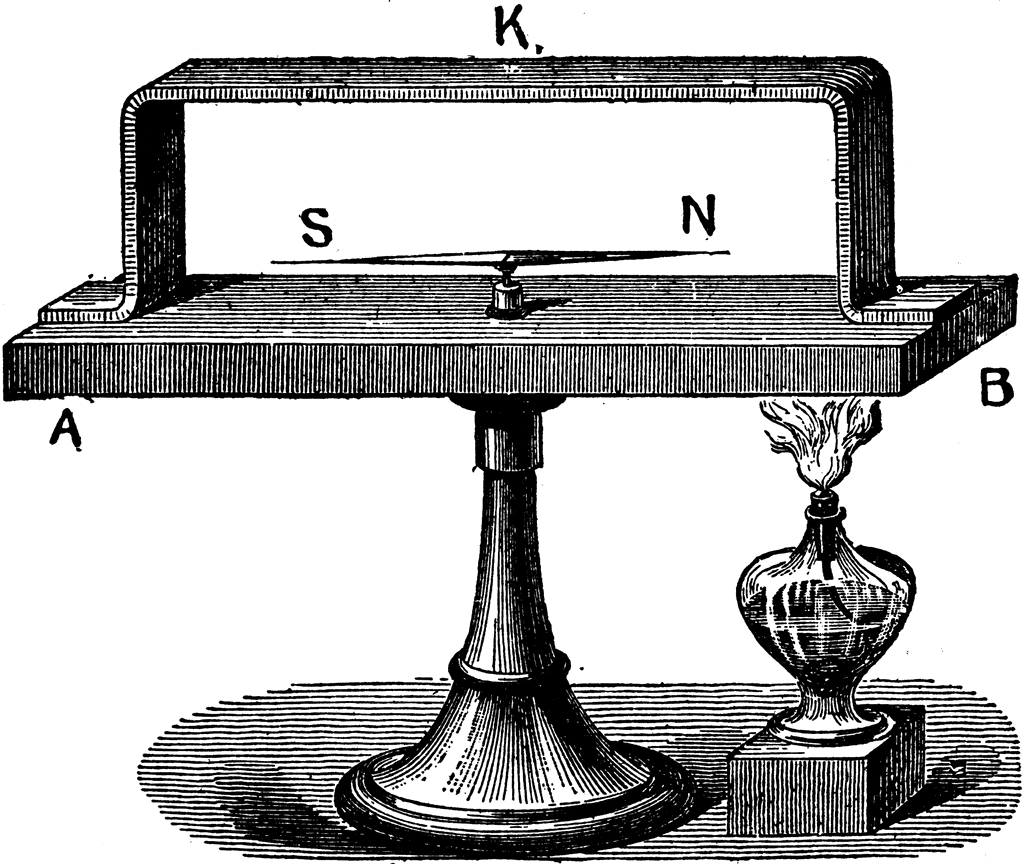
\includegraphics[width=\textwidth]{seebeck-experiment-black.png}
	\caption{Thomas Seebeck's original thermoelectricity experiment diagram \cite{seebeck-original}. A compass needle lies on top of one metal, underneath a bridge of a different metal (K), connected by two junctions and heated at one of these junctions.}
\end{figure}

\subsection{Nanocomposites}
Composite materials are combinations of two or more materials, forming a new structure with significantly different physical or chemical properties than its constituent parts. In a similar way, nanocomposites are the structuring of multiple materials, but at the nanoscale. As our nanocomposites are at a comparable size to the crystal lattices of their constituent materials, we can view nanocomposites as artificial defects in a larger crystal lattice. A simple example of a 2D nanocomposite, a copper-graphene superlattice, is pictured in \figref{superlattice}. Examining one layer of th0e superlattice, the material in bulk form would be a 3D crystal structure, but by constraining the layer thickness we have introduced a boundary defect. The periodic array of these boundary defects forms a new 3D artificial crystal, which we define as a superlattice, a nanocomposite.

\begin{figure}
	\label{fig:superlattice}
	\centering
	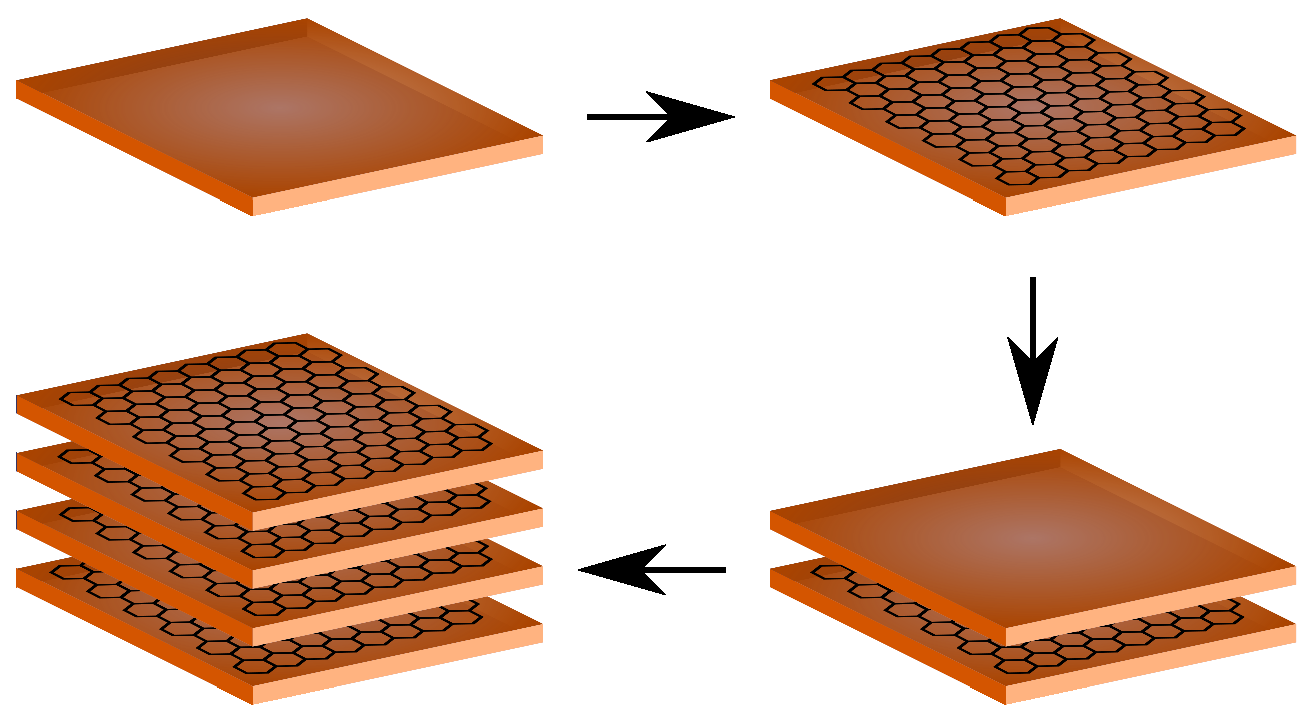
\includegraphics[width=\textwidth]{graphene-superlattice.eps}
	\caption{Superlattice of graphene and copper. Alternate layers of nanoscale copper and graphene are sandwiched together.}
\end{figure}

\subsection{Kinetic Theory}
\paragraph{Assumptions}

\section{Specific Theory}
% Details of exactly what you've done
% Tell a story, keep it concise, only explain what you need to
\subsection{Thermoelectric Theory}
\paragraph{Assumptions}

\section{Results and Analysis}
% Split into two sections if lengthy
% Explain all elements leading to the results
% Include key graphs, have minimal tables
% What do they show?

\section{Conclusion and Potential Development}
% Summarise results
% What else could be done?

% Link to your online repository
\url{https://github.com/kahlos/thermoelectrics}

% The {number} is related to the number of digits required for the references
\begin{thebibliography}{11}

\bibitem{modern-thermoelectrics}
D. M. Rowe,
\emph{Modern Thermoelectrics},
September 1983,
Holt-Technology,
ISBN:978-0835945936
\textbf{Page 12}

\bibitem{engine-efficiency}
M. L. Baglione,
\emph{Development of System Analysis Methodologies and Tools for Modeling and Optimizing Vehicle System Efficiency},
2007,
University of Michigan,
DOI:2027.42/57640
\textbf{Pages 52-54}

\bibitem{nanocomposite-zt}
R. Venkatasubramanian \emph{et al.},
\emph{Thin-film thermoelectric devices with high room-temperature figures of merit},
October 2001,
Nature, vol. 413, pp. 597-602,
DOI:10.1038/35098012

\bibitem{liu-review}
W. Liu \emph{et al.},
\emph{Recent advances in thermoelectric nanocomposites},
January 2012,
Nano Energy, vol. 1, iss. 1, pp. 42-56,
DOI:10.1016/j.nanoen.2011.10.001

\bibitem{crc-handbook}
G. A. Slack,
\emph{CRC Handbook of Thermoelectrics},
CRC Press (1995),
ISBN: 978-0849301469

\bibitem{minnich-review}
A. J. Minnich \emph{et al.}, \emph{Bulk nanostructured thermoelectric materials: current research and future prospects}, Energy Environ. Sci. 2, 466-479 (2009), DOI: 10.1039/B822664B
\end{thebibliography}


\appendix

\huge\textbf{Appendix}

\section{Further Questions and Thoughts}



\section{List of Assumptions}

\section{Further Reading}

\section{Tools and Software}

\section{Physical Data}

\section{Program Code}


\end{document}


%abbrivations list%
\acresetall
\ac{PGEC} - Exhibiting the properties of phonon scattering glasses and electron transmissive crystals
\ac{SSP} - The study of rigid matter (solids)